In the implementation, we take the elements $K \in T_h$, of the triangulation $T_h$ to be hexahedra.
\section{Numerical integration}
Evaluation of the integral values in \Cref{Linear1}, \Cref{Linear2} is performed using the \textit{Gaussian numerical quadrature}. A quadrature rule approximates the integral values by replacing the integral as a weighted sum of integrand values at specified points in the domain of integration. The Gaussian quadrature is constructed so that the approximation is exact for polynomials of degree 2\textit{n} - 1 (and less). This is acceptable, as our space $V_h$ is constructed using polynomials - see section \Cref{section:Vh} on the page \pageref{section:Vh}. We only need to take the value $n$ to be corresponding to the value of $p_m$ for the element $K_m$. The rule for both a 2-dimensional element face $\Gamma$, and a 3-dimensional cube $K$ is derived from a one-dimensional approximation (where the interval $\left[-1, 1\right]$ is a convention):
$$
\int_{-1}^1 f(x)\,dx = \sum_{i=1}^n w_i f(x_i),
$$
where the numbers $w_i > 0$ are the \textit{quadrature weights}, and the points (numbers in this case) $x_i$ are the \textit{quadrature points}, in the following way:
$$
\int_{\Gamma} f\lo\bfx\ro\,dx = \int_{-1}^{1}\int_{-1}^{1} f\lo x_1, x_2\ro\,dx \approx \sum_{i=1}^n\sum_{j=1}^n w_i w_j f\lo x_{1i}, x_{2j}\ro,
$$
$$
\int_{K} f\lo\bfx\ro\,dx = \int_{-1}^{1}\int_{-1}^{1}\int_{-1}^{1} f\lo x_1, x_2, x_3\ro\,dx \approx \sum_{i=1}^n\sum_{j=1}^n\sum_{k=1}^n w_i w_j w_k f\lo x_{1i}, x_{2j}, x_{3k}\ro,
$$
and transformation to a generic rectangular hexahedron is performed using the transformation in one dimension:
$$
\int_a^b f(x)\,dx \approx \frac{b-a}{2} \int_{-1}^1 f\left(\frac{b-a}{2}x + \frac{a+b}{2}\right)\,dx.
$$
Applying the Gaussian quadrature rule then results in the following one-dimensional approximation:
$$
\int_a^b f(x)\,dx \approx \frac{b-a}{2} \sum_{i=1}^n w_i f\left(\frac{b-a}{2}x_i + \frac{a+b}{2}\right).
$$
And the transformations in higher dimensions follow naturally. For $\Gamma = \left[a_1, b_1\right] \times \left[a_2, b_2\right]$ we have:
$$
\int_{\Gamma} f(x)\,d\bfx \approx \frac{b_2-a_2}{2}\frac{b_1-a_1}{2} \sum_{i=1}^n \sum_{j=1}^n w_i w_j f\lo\frac{b_1-a_1}{2}x_i + \frac{a_1+b_1}{2},\frac{b_2-a_2}{2}x_j + \frac{a_2+b_2}{2}\ro.
$$
Taking now e.g. \Cref{Linear1}, and notation for quadrature points and weights, we can write (omitting the operand $\bfx = \lo x_1, x_2, x_3\ro$):
\begin{align}
a_{lm} & =  \sum_{K^i \in T_h}\int_{K^i} \mrvhl \mrvhm, \\
a_{lm} & := \sum_{K^i \in T_h}\int_{K^i} f\lo\mrvhl, \mrvhm\ro , \\
a_{lm} & \approx \sum_{K^i \in T_h} \sum_{\bfj=\overrightarrow{1}}^{\overrightarrow{n}} f\lo\mrvhl\lo\bfx_{\bfj}^i\ro, \mrvhm\lo\bfx_{\bfj}^i\ro\ro\,w_{\bfj},\label{Final_Integration_Fn}
\end{align}
where $\bfj$ is a multi-index used in sum over (volumetric) quadrature points $\bfx_{\bfj}^i \in K^i$.
Similarly for the right-hand side (\Cref{Linear2}):
\begin{align}
b_{l} & =  \sum_{K^i \in T_h}\int_{K^i} \left[{\mrPsi_h}^{k} + \tau\mrS + \tau\mrA\lo{\mrPsi_h^{k}}\ro \lo\nabla \cdot \mrvhl\ro\right] \mrvhl\\
\nonumber & - \sum_{\Gamma_{ij}\in\Gamma_I} \int_{\Gamma_{ij}}\mrH\lo{\mrPsi_h^{k}}|_{ij}, {\mrPsi_h^{k}}|_{ji}, \bfn_{ij}\ro \mrvhl\\
\nonumber& - \sum_{\Gamma_{ij}\in\Gamma_B} \int_{\Gamma_{ij}} \mrH\lo{\mrPsi_h^{k}}|_{ij}, \overline{{\mrPsi_h^{k}}|_{ji}}, \bfn_{ij}\ro \mrvhl,\\
\label{Final_Integration_Fn_b}   b_{l} & := \sum_{K^i \in T_h}\int_{K^i} g\lo\mrvhl\ro - \sum_{\Gamma_{ij}\in\Gamma_I} \int_{\Gamma_{ij}}g^{'}\lo\mrvhl\ro - \sum_{\Gamma_{ij}\in\Gamma_B} \int_{\Gamma_{ij}} g^{''}\lo\mrvhl\ro \\
b_{l} & \approx \sum_{K^i \in T_h} \sum_{\bfj=\overrightarrow{1}}^{\overrightarrow{n}} g\lo\mrvhl\lo\bfx_{\bfj}^i\ro\ro\,w_{\bfj}\\
\nonumber & -  \sum_{\Gamma_{ij}\in\Gamma_I} \sum_{\bfj_f=\overrightarrow{1}}^{\overrightarrow{n_f}} g^{'}\lo\mrvhl\lo\bfx^{ij}_{\bfj_{f}}\ro\ro\,w_{\bfj_{f}}\\
\nonumber & -  \sum_{\Gamma_{ij}\in\Gamma_B} \sum_{\bfj_{f}=\overrightarrow{1}}^{\overrightarrow{n_f}} g^{''}\lo\mrvhl\lo\bfx^{ij}_{\bfj_{f}}\ro\ro\,w_{\bfj_{f}},
\end{align}
where in addition to $\bfj$ as explained before, $\bfj_{f}$ is a multi-index used sum over face quadrature points $\bfx_{\bfj_f}^{ij} \in \Gamma_{ij}$. Based on this, we can define
\begin{align}
	\label{singleNumIntA}   a_{lmi \bfj} & =  f\lo\mrvhl\lo\bfx^i_{\bfj}\ro, \mrvhm\lo\bfx^i_{\bfj}\ro\ro\,w_{\bfj},\\
	\label{singleNumIntB}   b_{li \bfj} & =  g\lo\mrvhl\lo\bfx^i_{\bfj}\ro\ro\,w_{\bfj},\\
	\label{singleNumIntBface}  b^{'}_{lij \bfj_f} & =  \left\{\begin{array}{c} g^{'}\lo\mrvhl\lo\bfx^{ij}_{\bfj_f}\ro\ro\,w_{\bfj}\ \ \text{if}\ \Gamma_{ij}\in \Gamma_I \\ g^{''}\lo\mrvhl\lo\bfx^{ij}_{\bfj_f}\ro\ro\,w_{\bfj}\ \ \text{if}\ \Gamma_{ij}\in \Gamma_B \end{array}\right. .
\end{align}

\section{Assembling the algebraic problem}
Now we have a clear expression how to evaluate the integral values \Cref{Linear1}, \Cref{Linear2} using \Cref{singleNumIntA}, \Cref{singleNumIntB}, \Cref{singleNumIntBface}, but we need to construct the matrix $A$ (\Cref{Linear3}), and the right-hand-side vector $b$ (\Cref{Linear4}) in an effective manner.
This is generally achieved through a \textit{element-wise} assembling of these structures. Key to this is to create a data structure that identifies for a particular element $K^i$ all the test functions $\mrvhl$ that make sense to be evaluated (have non-empty support) on $K^i$, i.e. we are looking for the set
\be
\mrvh \lo K^i \ro = \left\{\mrvh \in V_h : supp\lo\mrvh\ro \cap K^i \neq \emptyset \right\},
\ee
and do the same for the faces $\Gamma_i$ (both boundary, and internal):
\be
\mrvh \lo \Gamma_i \ro = \left\{\mrvh \in V_h : supp\lo\mrvh\ro \cap \Gamma_i \neq \emptyset \right\}.
\ee
Now the assembling procedure looks like this:\\
\begin{algorithm}[H]
    \# 1 - Loop over elements\\
    \ForEach{$K^i\in T_h$}{
       \KwData{Quadrature points $\left\{\bfx^i_1, ..., \bfx^i_{\bfn}\right\}$}
       \KwData{Jacobian of the mapping $J_{K^i}$ mapping the reference element (unit cube) to the actual element}
       \KwData{Quadrature weights $\left\{w_1, ..., w_{\bfn}\right\}$}
                   \# Loop over quadrature points\\
       \ForEach{$\bfj \in \left\{1, ..., \bfn\right\}$}{
           \textbf{Set: }$\lo JxW\ro_{\bfj} = J_{K^i} \times w_{\bfj}$\\
            \# Loop over test functions\\
        \ForEach{$v\in v_h \lo {K^i} \ro$}{
       \KwData{$l$ - index of $v$ in the global system, i.e. row in \Cref{Linear3} - \Cref{Linear5}}
                        \# Loop over basis functions\\
            \ForEach{$u\in v_h \lo {K^i} \ro$}{
       \KwData{$m$ - index of $u$ in the global system, i.e. column in \Cref{Linear3}}
                
                        $a_{lm}\ \ +=\ \ \lo JxW\ro_{\bfj} \ a_{lmi \bfj}$
                    }

                $b_{l}\ \ +=\ \ \lo JxW\ro_{\bfj} \ b_{li \bfj}$
        }                
        }
    }
\ \\
        \# 2 - Loop over faces\\
        \ForEach{$\Gamma_{ij}\in T_h$}{
            \KwData{Quadrature points $\left\{\bfx^{ij}_1, ..., \bfx^{ij}_{\bfn_f}\right\}$}
            \KwData{Jacobian of the mapping $J_{K^i} = J_{K^-}$ mapping the reference face (unit square) to the actual face, where $K^i, K^j$ are elements adjacent to $\Gamma_{ij}$ if this is an internal face, or $K^i = K^j$ if this is a boundary face.}
            \KwData{Quadrature weights $\left\{w_1, ..., w_{\bfn_f}\right\}$}
            \# Loop over quadrature points\\
            \ForEach{$\bfj_f \in \left\{1, ..., \bfn_f\right\}$}{
                \textbf{Set: }$\lo JxW\ro_{\bfj_f} = J_{K^i} \times w_{\bfj_f}\ $ \# Here it does not matter if we choose $J_{K^i}$ or $J_{K^j}$\\
                \# Loop over test functions\\
                \ForEach{$v\in v_h \lo K^i \ro$}{
                    \KwData{$l$ - index of $v$ in the global system, i.e. row in \Cref{Linear3} - \Cref{Linear5}}
                    
                    $b_{l}\ \ +=\ \ \lo JxW\ro_{\bfj_f} \ b^{'}_{lij \bfj_f}$
                }
            }
        }
\caption{Assembling of the algebraic problem \Cref{Alg}}
\label{algorithm:singleTimeStep}
\end{algorithm}
An important remark needs to be added here, with respect to the fact, that we aim for a distributed computation. As stated before, the domain decomposition approach leads to each of the processors $P_i \in \left\{P_0, ..., P_N\right\}$ of the total number of processors employed for the computation owning only a subset of elements $\left\{K \in T\right\}_i$. If the processor $P_i$ did not have any data about other elements, we would not be able to perform the evaluation involving $b^{'}$ defined in \Cref{singleNumIntBface}, or more precisely $g^{'}$ defined in \Cref{Final_Integration_Fn_b} as the values ${\mrPsi_h^{k}}|_{ji}$ for faces $\Gamma_{ij}$ of elements from $\left\{K \in T\right\}_i$ will not always be there.
\paragraph{}
To amend this situation, in the distributed triangulation, each processor holds not only the mesh element data it owns, but also data for mesh elements it needs - in Discontinuous Galerkin method, for exactly the purposes of internal face integral evaluation described in the previous paragraph. This data is called \textit{ghost elements}, or \textit{ghost cells}, as these are only copies provided by other processors which own the particular elements. This is illustrated in \Cref{figure:ghost}, which is the same case of distributed triangulation as shown in \Cref{figure:domainDecomposition}.

\begin{figure}[H]
		\begin{center}
			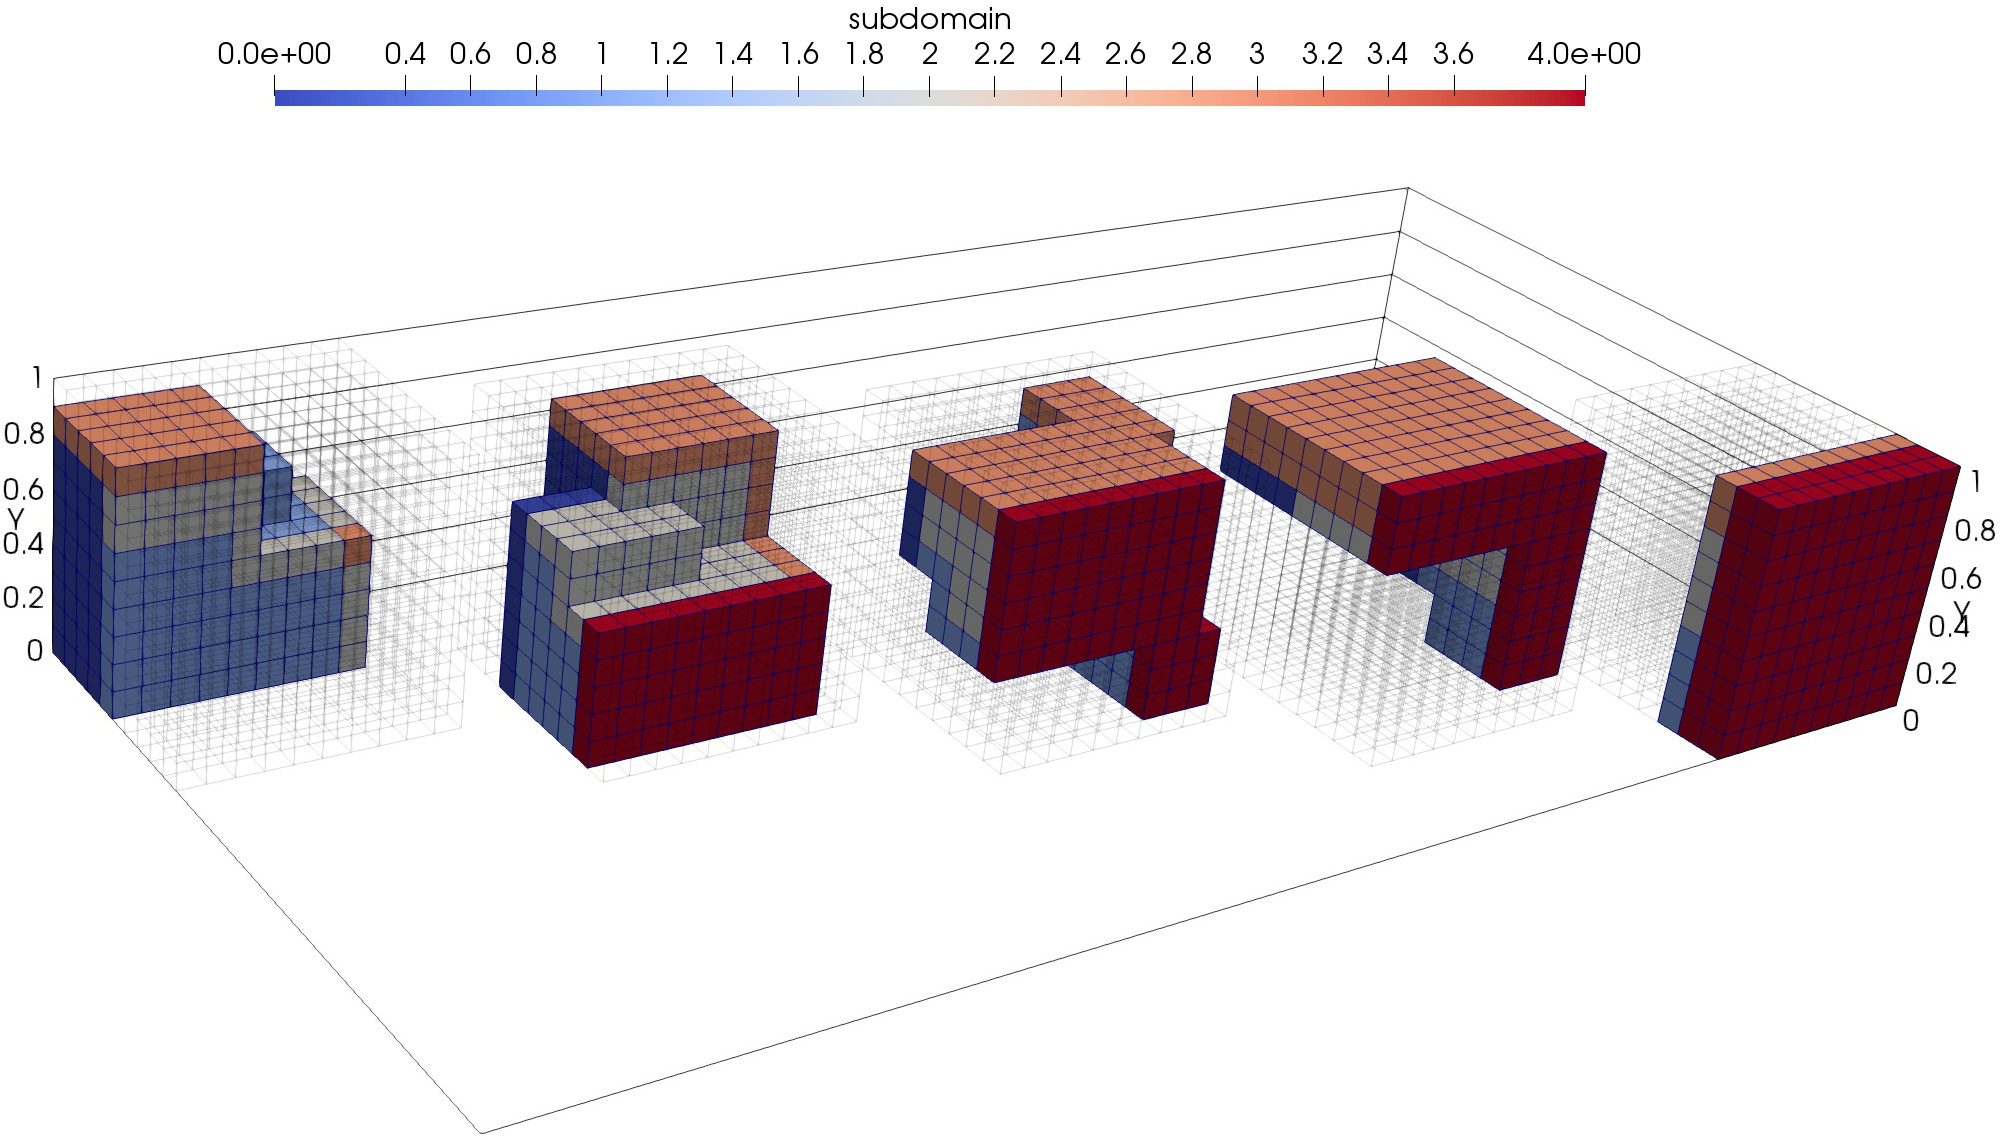
\includegraphics[width=0.78\textwidth]{img/mesh/cube-NONperiodic,ghost.jpg}
			\vspace{-2mm}
		\caption{Processor-owned elements (0..4 left to right), with color-coded ghost elements from other processors.}
		\label{figure:ghost}
		\end{center}
	\end{figure}\vspace{-5mm}

\paragraph{}
Note that in the described algorithm, and also with respect to the remarks in the previous paragraphs, periodic boundary conditions are not specifically handled, as they are only a technically more complex case of internal faces (both from the perspective of necessity of utilizing ghost cells, and from the perspective of evaluating $b_{l}$ in \Cref{algorithm:singleTimeStep}.